\providecommand{\devnum}[1]{#1}

\section{Introduction}
\label{sec:intro}

A shared execution service runs jobs on behalf of many users on a fixed pool of $k$ servers. A job that has started is not interrupted: it runs until it finishes or until it reaches a per-job time limit $L$. Serverless function platforms, build and test farms for continuous integration, batch inference queues, and the judging back ends of programming-assignment platforms are all organised this way \cite{wasik2018ojsurvey}. Operators document the consequence themselves: a contest judging system recommends one judging host per twenty teams and notes that with fewer hosts the waiting time grows \cite{domjudge_manual}, and the maintainers of a university autograder replayed the busiest four hours before a common deadline and found that one submission looping until its resource limit took a grader out of circulation and delayed the graders behind it \cite{peveler2019sandbox}; their replay compresses that window, a method we argue against in Section~\ref{sec:limits} and replace by overlaying whole class-terms. Two properties of the offered load make such a service slow down when it is used most. Arrivals follow an external calendar, so they are neither stationary nor independent; the same concentration near a fixed cutoff has been measured directly \cite{konig2005deadline,alfi2007deadline,alfi2009deadline}. And job costs are concentrated in a small fraction of jobs: on the serverless invocation trace we use \cite{azure2021trace,zhang2021harvested}, the longest \devnum{1\%} of invocations account for \devnum{44\%} of the total work, and on the main judging trace, after the analysis service cap is applied, the longest \devnum{1\%} still account for \devnum{37.5\%}, and \devnum{27.5\%} on the second. A few very long jobs therefore sit in front of many short ones exactly when the queue is longest.

The mechanism we exploit is visible in a queue of three jobs on one server (Figure~\ref{fig:threejob}). Job $A$ loops forever and is stopped by the 60-second limit; jobs $B$ and $C$ take 0.2 seconds each. In arrival order the mean wait is 40.1 seconds; shortest first it is 0.2 seconds, at a cost of 0.4 seconds to $A$. The server performs the same total work in both orders. The three numbers are arithmetic; we have not simulated anything yet, and they rest on one assumption: that the scheduler knows, before $A$ starts, that $A$ will be long. That assumption raises three questions, and the paper is organised around them. Can the cost of a job be estimated at the moment it arrives, from history that is causally visible at that instant? Given estimates, what should a non-preemptive scheduler rank by? And what happens to an individual job when the estimates are wrong?

% Figure: the three-job example of Section 1, drawn as two timelines.
% Every number in it is the arithmetic stated in the text of Section~\ref{sec:intro}:
% A = 60 s (stopped at the limit L = 60 s), B = C = 0.2 s, one server, all three
% present at t = 0.  FCFS waits 0 / 60.0 / 60.2 (mean 40.1 s); shortest-first waits
% 0.4 / 0 / 0.2 (mean 0.2 s).  No new computation: this is the paragraph above it.
\begin{figure}[htbp]
\centering
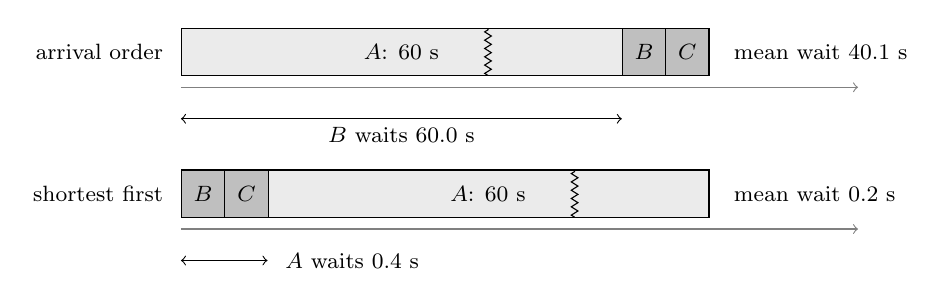
\begin{tikzpicture}[x=1cm,y=1cm,font=\footnotesize]
  % ---- style
  \tikzset{
    jobbox/.style={draw,minimum height=6mm,inner sep=2pt},
    lbl/.style={anchor=east,inner sep=2pt},
  }
  % ---- row 1: arrival order
  \node[lbl] at (-0.15,0.3) {arrival order};
  \draw[->,gray] (0,-0.15) -- (8.6,-0.15);
  \node[jobbox,fill=black!8,minimum width=5.6cm,anchor=west] (a1) at (0,0.3) {};
  \node at (2.8,0.3) {$A$: 60 s};
  % break marks inside A
  \draw[decorate,decoration={zigzag,segment length=3pt,amplitude=1.2pt}] (3.9,0.0) -- (3.9,0.6);
  \node[jobbox,fill=black!25,minimum width=0.55cm,anchor=west] (b1) at (5.6,0.3) {$B$};
  \node[jobbox,fill=black!25,minimum width=0.55cm,anchor=west] (c1) at (6.15,0.3) {$C$};
  \node[anchor=west] at (6.9,0.3) {mean wait 40.1 s};

  % ---- row 2: shortest first
  \node[lbl] at (-0.15,-1.5) {shortest first};
  \draw[->,gray] (0,-1.95) -- (8.6,-1.95);
  \node[jobbox,fill=black!25,minimum width=0.55cm,anchor=west] (b2) at (0,-1.5) {$B$};
  \node[jobbox,fill=black!25,minimum width=0.55cm,anchor=west] (c2) at (0.55,-1.5) {$C$};
  \node[jobbox,fill=black!8,minimum width=5.6cm,anchor=west] (a2) at (1.1,-1.5) {};
  \node at (3.9,-1.5) {$A$: 60 s};
  \draw[decorate,decoration={zigzag,segment length=3pt,amplitude=1.2pt}] (5.0,-1.8) -- (5.0,-1.2);
  \node[anchor=west] at (6.9,-1.5) {mean wait 0.2 s};

  % ---- waits
  \draw[<->] (0,-0.55) -- node[below,inner sep=3pt] {$B$ waits 60.0 s} (5.6,-0.55);
  \draw[<->] (0,-2.35) -- (1.1,-2.35);
  \node[anchor=west,inner sep=2pt] at (1.25,-2.35) {$A$ waits 0.4 s};
\end{tikzpicture}
\caption{The three-job example of Section~\ref{sec:intro} on one server: $A$ is
stopped at the per-job limit $L = \devnum{60}$ s, $B$ and $C$ take
\devnum{0.2} s each, and all three are present at $t = 0$. The boxes are
schematic, not to scale, and the zigzag marks the elided part of $A$. The two
orders execute the same total work; reordering moves \devnum{60} seconds of
waiting off $B$ and $C$ and puts \devnum{0.4} seconds onto $A$. Source: the
arithmetic stated in the text, not a measurement.}
\label{fig:threejob}
\end{figure}


On the first, arrival-time history is enough to tell the heavy jobs from the rest on all three platforms. We compare three families of predictor on one split and one visibility protocol --- tabular models \cite{ke2017lightgbm}, a sequence model over each user's history, and a heterogeneous graph neural network over the user, task and assignment entities \cite{schlichtkrull2018rgcn} --- and the graph model does not improve on the tabular one: removing every edge, and then permuting the edges at random, leaves its classification scores where they were, which places the signal in each entity's own history rather than in the relational structure. We report that as a property of this prediction task and not of relational models (Section~\ref{sec:prediction}). On the second question, we rank by estimated conditional expected cost $\mathbb{E}[C \mid x]$ rather than by a log-scale prediction, whose back-transform generally differs from the arithmetic mean; the single-server interchange argument motivates that choice without establishing optimality for multiple servers, arbitrary arrivals or deadline-window percentiles. Errors in the fitted score are asymmetric, treating a heavy job as light and letting it run first being the expensive mistake by about an order of magnitude, which diagnoses that score rather than establishing a universal loss-function comparison (Sections~\ref{sec:scheduling} and~\ref{sec:exp_rank}).

The third question is the one an operator will ask first. Ordering by prediction improves the bulk of the distribution and can damage the tail: in our busiest configuration one job waited almost a hundred job-limits longer than it would have under first-come first-served (Section~\ref{sec:exp_guard}). Robustness results in the scheduling-with-predictions literature usually bound an expectation against an optimal or shortest-remaining-processing-time reference, and the constant-factor ones require the prediction error to be bounded multiplicatively, which is not a property anyone can promise about a deployed predictor \cite{scully2022uniform,mitzenmacher2025queueing}. There are exceptions on single axes. One line bounds the maximum stretch over all jobs on a preemptive machine, which is not an expectation \cite{zhao2025fairpredictions}; another bounds a request's latency in a stationary light-tailed queue against the workload the system holds at the request's boosted arrival instant, using the work that overtakes it \cite{yu2024boost,yu2025twotraffics}; read on a sample path that is close to a bound against first-come first-served, but it is not the form those papers state. What we do not find is the conjunction: a first-come first-served reference, stated per job, on an arbitrary arrival sequence with arbitrary predictions, non-preemptive, on $k$ servers, and enforced online around whatever policy is underneath instead of analysed for one fixed policy. We change the reference point instead of strengthening the assumption, and bound, for each job separately, how much longer it waits than it would have waited under first-come first-served on the same arrival sequence, assuming nothing about the arrival process and nothing about prediction quality. The mechanism is an overtake budget: for every waiting job we account the total work of later-ordered jobs that have completed while it waited, and at each dispatch decision the smallest-ranked waiting job whose account reaches its current budget takes precedence. The guard wraps an arbitrary base scheduler, including a learned one, and touches only the dispatch decision. It is one mechanism with one parameter that matters for the promise, a cap $B_{\max}$ on the budget; what the budget does below that cap is a design freedom that changes how much of the base policy's benefit survives and which jobs pay for it, and changes the promise not at all.

We budget work rather than count overtakes because the identity puts the guarantee in units of work: a job's delay relative to first-come first-served equals its net overtaken work divided by $k$, to within $(2-2/k)L$, for every non-preemptive work-conserving $k$-server policy and every arrival sequence. The identity does not refer to the policy and it cuts both ways, which is what makes a work budget the right currency and a bound on the \emph{number} of overtakes the wrong one. The guarantee is denominated in units of $L$, so the uniform certificate is most informative when $L$ is comparable to the waits an operator cares about; a computing farm whose jobs run for days illustrates a certificate too coarse for those waits, which does not rule out tighter guarantees for a restricted policy or workload.

We make four contributions.

\begin{itemize}
  \item The net-overtake identity just stated, with the constant $(2-2/k)L$ shown to be an exact supremum, approached and never attained, and a corollary in the other direction: any per-job guarantee of this kind bounds the overtaken work, up to an additive $O(kL)$.
  \item An overtake-budget guard. It wraps any base scheduler and bounds every job's wait against first-come first-served, for $k$ servers, arbitrary arrivals and arbitrary predictions. The bound reads the budget only through a cap: any budget rule with $0 \le \mathrm{budget} \le B_{\max}$ gives the same guarantee, so the operator sets $B_{\max} = k(G - (3-2/k)L)$ from a promise $G$ in seconds, with no data, and is then free in how the budget is spent below it. The additive constant $(3-2/k)L$, beyond the budget term, is an exact supremum, never attained, and it grows with $k$ from $L$ at $k = 1$ towards $3L$; no analysis of this mechanism can improve it. One shape of budget, the one whose allowance grows with the wait a job has already had, carries a multiplicative bound as well. We state which assumptions can be dropped, and show by counterexample that work conservation cannot.
  \item A comparison of cost predictors on causally visible history, covering tabular, sequence and heterogeneous graph models, with two conclusions that carry into the scheduler: expected-cost ordering performs better than the log-scale alternative in the reported source-clock comparisons, and the fitted score is more sensitive to severe underestimates. Separate conservative and static controls examine the availability of that history in a replayed queue.
  \item An evaluation on real logs from two programming-assignment judging platforms \cite{codebench_dataset,accoding2024} and a serverless invocation trace \cite{azure2021trace}, with every simulated job checked against the theoretical bound, and two applicability conditions read off six workloads, most of which fail one or the other: the uniform certificate is too coarse where the waits are short relative to $L$, and there is little to exploit where costs are not concentrated \cite{netbatch2012trace,shai2014netbatch,taskcluster_docs,treeherder_docs}. Section~\ref{sec:exp_cross} reads both conditions off the six in numbers and Section~\ref{sec:limits} states what they rule out.
\end{itemize}

Four qualifications hold over everything reported below, and each is stated where the
numbers are. The judging logs supply recorded execution demand and do not identify a
historical shared queue, so the pooled capacity and the replayed waiting times are
experimental constructions of ours (Section~\ref{sec:data}); a capacity sweep and an
executing timed-work service test the mechanism under fixed offered work, and the
physical guard, while it follows the dispatch rule, has a higher p99 than the separately
timed first-come first-served run and does not reproduce the ideal simulator job by job
(Section~\ref{sec:exp_physical}). Every figure quoted in this paper is a development
figure: the sealed parts of three traces, the main one's three terms among them, will be
opened once after the method, the parameters and the primary metric have been frozen, and
their numbers will be reported separately (Section~\ref{sec:sealed}). The empirical
headline uses conservative history visibility, under which Guard($\devnum{600}$) closes
$\devnum{0.429}$ of the FCFS-to-SJF gap at the busiest load, with interval
$\devnum{[0.357, 0.533]}$, against $\devnum{0.801}$ under the original result clock, which
we retain as an optimistic reference (Section~\ref{sec:exp_visibility}). And the
guarantee is per job and additive, so a guarded run may still have a worse quantile than
first-come first-served, by at most the promise (Section~\ref{sec:limits}).
% Source: outputs/dev_visibility/visibility_comparison.csv, level=2,
% Guard(600) and Guard(600)-original, gap_closed and gap_closed_lo/hi.
% Ninth pass: the detailed numeric preview that stood here --- the predictor AUROCs, the
% two asymmetry fractions, the worst unguarded excess in seconds and the applicability
% read-off --- is now carried only where it is derived, in Sections 4, 7, 8.2, 8.4 and
% 8.7 and in Section 9; prechecks/heldout_scope/heldout_scope.md, G1 and G2--G3, is the
% source of the sealed-scope sentence, which Section 7.5 also carries.

Section~\ref{sec:related} places the paper in the literature and Section~\ref{sec:model} states the model, the visibility protocol and the metrics. Sections~\ref{sec:prediction} and~\ref{sec:scheduling} give the cost predictors and the scheduler, Section~\ref{sec:theory} the identity, the per-job bounds and their tightness, and Section~\ref{sec:data} the traces. Section~\ref{sec:experiments} reports the experiments and Section~\ref{sec:limits} the limitations; the deferred proofs and the tightness constructions are Supplementary Sections~S4 and~S8.
